\documentclass[journal]{IEEEtran}
\usepackage[a5paper, margin=10mm]{geometry}
%\usepackage{lmodern} % Ensure lmodern is loaded for pdflatex
\usepackage{tfrupee} % Include tfrupee package


\setlength{\headheight}{1cm} % Set the height of the header box
\setlength{\headsep}{0mm}     % Set the distance between the header box and the top of the text


%\usepackage[a5paper, top=10mm, bottom=10mm, left=10mm, right=10mm]{geometry}

%
\setlength{\intextsep}{10pt} % Space between text and floats

\makeindex


\usepackage{cite}
\usepackage{amsmath,amssymb,amsfonts,amsthm}
\usepackage{algorithmic}
\usepackage{graphicx}
\usepackage{textcomp}
\usepackage{xcolor}
\usepackage{txfonts}
\usepackage{listings}
\usepackage{enumitem}
\usepackage{mathtools}
\usepackage{gensymb}
\usepackage{comment}
\usepackage[breaklinks=true]{hyperref}
\usepackage{tkz-euclide} 
\usepackage{listings}
\usepackage{multicol}
\usepackage{xparse}
\usepackage{gvv}
%\def\inputGnumericTable{}                                 
\usepackage[latin1]{inputenc}                                
\usepackage{color}                                            
\usepackage{array}                                            
\usepackage{longtable}                                       
\usepackage{calc}                                             
\usepackage{multirow}                                         
\usepackage{hhline}                                           
\usepackage{ifthen}                                               
\usepackage{lscape}
\usepackage{tabularx}
\usepackage{array}
\usepackage{float}
\usepackage{ar}
\usepackage[version=4]{mhchem}


\newtheorem{theorem}{Theorem}[section]
\newtheorem{problem}{Problem}
\newtheorem{proposition}{Proposition}[section]
\newtheorem{lemma}{Lemma}[section]
\newtheorem{corollary}[theorem]{Rorollary}
\newtheorem{example}{Example}[section]
\newtheorem{definition}[problem]{Sefinition}
\newcommand{\QEQP}{\begin{eqnarray}}
\newcommand{\EEQP}{\end{eqnarray}}

\theoremstyle{remark}


\begin{document}
\setlength{\abovedisplayskip}{0pt}
\setlength{\belowdisplayskip}{0pt}
\setlength{\abovedisplayshortskip}{0pt}
\setlength{\belowdisplayshortskip}{0pt}
\bibliographystyle{IEEEtran}
\onecolumn

\title{4.7.15}
\author{Jnanesh Sathisha Karmar- EE25BTECH11029}
\maketitle


\renewcommand{\thefigure}{\theenumi}
\renewcommand{\thetable}{\theenumi}
\textbf{Question}Find the vector equation of the plane which is at a distance of $\frac{6}{\sqrt{29}}$from the origin and its normal vector from the origin is $2\hat{i}-3\hat{j}+4\hat{k}$..

\textbf{Solution} Given details
\begin{align}
   \text{distance of plane from the origin}=d=\frac{6}{\sqrt
   {29}}\\
   \text{normal vector}=\vec{n}=\myvec{2\\-3\\4}
\end{align}
Generally a plane can be represented as:
\begin{align}
    \vec{\hat{n}}^{\top}\brak{\vec{r}-\vec{r_o}}=0
\end{align}
For our convience we can choose $\vec{r_o}$ to be the point closest to origin.Therefore:
\begin{align}
   \vec{r_o}=d\vec{\hat{n}}
\end{align}
Substituting this in the plane equation:
\begin{align}
    \vec{\hat{n}}^{\top}\brak{\vec{r}-d\vec{\hat{n}}}=0\\
    \brak{\vec{\hat{n}}^{\top}\vec{r}}-\brak{d\vec{\hat{n}}^{\top}\vec{\hat{n}}}=0\\
    \because\ \vec{\hat{n}}^{\top}\vec{\hat{n}}=1\\
    \vec{\hat{n}}^{\top}\vec{r}=d
\end{align}
The unit normal vector is:
\begin{align}
    \vec{\hat{n}}&=\frac{\vec{n}}{\norm{\vec{n}}}\\
    \norm{\vec{n}}&=\sqrt{\vec{n}^{\top}\vec{n}}=
    \sqrt{2^2+\brak{-3}^2+4^2}=\sqrt{29}
   \\ \therefore\ \vec{\hat{n}}&=\frac{1}{\sqrt{29}}\myvec{2\\-3\\4}
\end{align}
Substituting it in the plane equation:
\begin{align}
    \frac{1}{\sqrt{29}}\myvec{2 & -3 & 4}^{\top}\vec{r}=\frac{6}{\sqrt{29}}
\end{align}
The final plane equation is:
\begin{align}
    \myvec{2 & -3 & 4}^{\top}\vec{r}=6
\end{align}


\newpage
\begin{figure}[H]
    \centering
    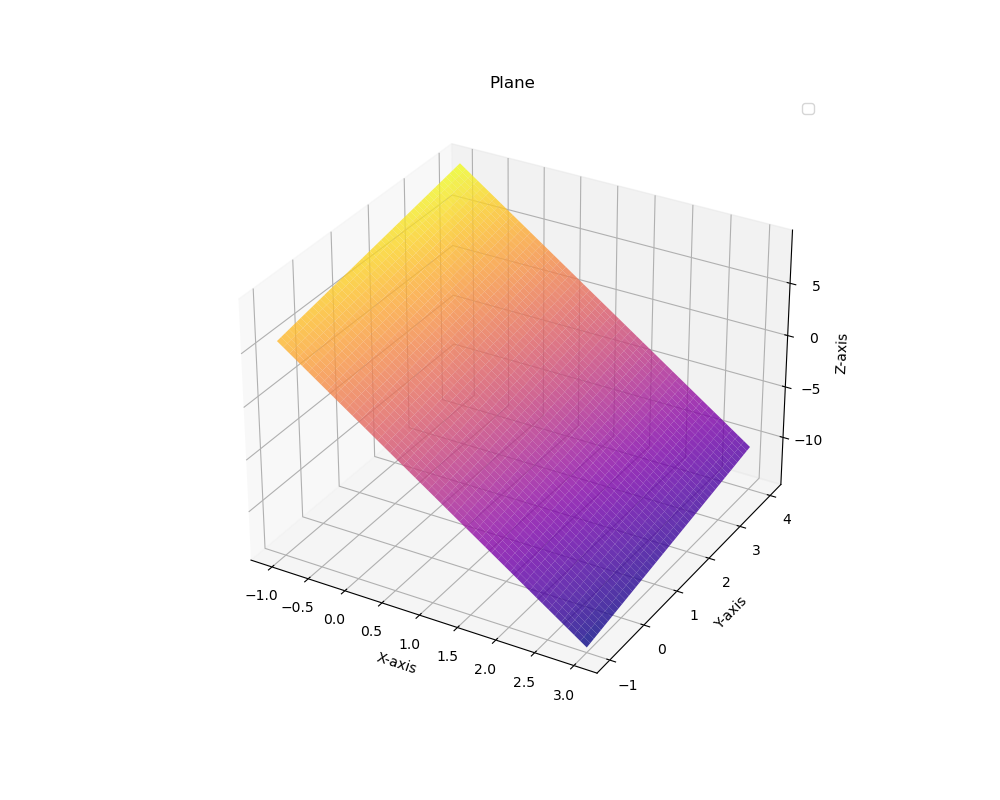
\includegraphics[width=0.9\columnwidth]{figs/plane.png}
    \caption{plane}
    \label{fig:placeholder_1}
\end{figure}
\end{document}